% Options for packages loaded elsewhere
\PassOptionsToPackage{unicode}{hyperref}
\PassOptionsToPackage{hyphens}{url}
%
\documentclass[
  ignorenonframetext,
  aspectratio=169]{beamer}
\usepackage{pgfpages}
\setbeamertemplate{caption}[numbered]
\setbeamertemplate{caption label separator}{: }
\setbeamercolor{caption name}{fg=normal text.fg}
\beamertemplatenavigationsymbolsempty
% Prevent slide breaks in the middle of a paragraph
\widowpenalties 1 10000
\raggedbottom
\setbeamertemplate{part page}{
  \centering
  \begin{beamercolorbox}[sep=16pt,center]{part title}
    \usebeamerfont{part title}\insertpart\par
  \end{beamercolorbox}
}
\setbeamertemplate{section page}{
  \centering
  \begin{beamercolorbox}[sep=12pt,center]{part title}
    \usebeamerfont{section title}\insertsection\par
  \end{beamercolorbox}
}
\setbeamertemplate{subsection page}{
  \centering
  \begin{beamercolorbox}[sep=8pt,center]{part title}
    \usebeamerfont{subsection title}\insertsubsection\par
  \end{beamercolorbox}
}
\AtBeginPart{
  \frame{\partpage}
}
\AtBeginSection{
  \ifbibliography
  \else
    \frame{\sectionpage}
  \fi
}
\AtBeginSubsection{
  \frame{\subsectionpage}
}
\usepackage{lmodern}
\usepackage{amssymb,amsmath}
\usepackage{ifxetex,ifluatex}
\ifnum 0\ifxetex 1\fi\ifluatex 1\fi=0 % if pdftex
  \usepackage[T1]{fontenc}
  \usepackage[utf8]{inputenc}
  \usepackage{textcomp} % provide euro and other symbols
\else % if luatex or xetex
  \usepackage{unicode-math}
  \defaultfontfeatures{Scale=MatchLowercase}
  \defaultfontfeatures[\rmfamily]{Ligatures=TeX,Scale=1}
\fi
\usetheme[]{Frankfurt}
\usecolortheme{beaver}
% Use upquote if available, for straight quotes in verbatim environments
\IfFileExists{upquote.sty}{\usepackage{upquote}}{}
\IfFileExists{microtype.sty}{% use microtype if available
  \usepackage[]{microtype}
  \UseMicrotypeSet[protrusion]{basicmath} % disable protrusion for tt fonts
}{}
\makeatletter
\@ifundefined{KOMAClassName}{% if non-KOMA class
  \IfFileExists{parskip.sty}{%
    \usepackage{parskip}
  }{% else
    \setlength{\parindent}{0pt}
    \setlength{\parskip}{6pt plus 2pt minus 1pt}}
}{% if KOMA class
  \KOMAoptions{parskip=half}}
\makeatother
\usepackage{xcolor}
\IfFileExists{xurl.sty}{\usepackage{xurl}}{} % add URL line breaks if available
\IfFileExists{bookmark.sty}{\usepackage{bookmark}}{\usepackage{hyperref}}
\hypersetup{
  pdftitle={Centers of diversity of crops and wild genetic diversity},
  pdfauthor={Deependra Dhakal},
  hidelinks,
  pdfcreator={LaTeX via pandoc}}
\urlstyle{same} % disable monospaced font for URLs
\newif\ifbibliography
\setlength{\emergencystretch}{3em} % prevent overfull lines
\providecommand{\tightlist}{%
  \setlength{\itemsep}{0pt}\setlength{\parskip}{0pt}}
\setcounter{secnumdepth}{-\maxdimen} % remove section numbering
\usepackage{booktabs}
\usepackage{longtable}
\usepackage{array}
\usepackage{multirow}
\usepackage{wrapfig}
\usepackage{float}
\usepackage{colortbl}
\usepackage{pdflscape}
\usepackage{tabu}
\usepackage{threeparttable}
\usepackage{threeparttablex}
\usepackage[normalem]{ulem}
\usepackage{makecell}
\usepackage{xcolor}
\usepackage{tikz} % required for image opacity change
\usepackage[absolute,overlay]{textpos} % for text formatting

% this font option is amenable for beamer
\setbeamerfont{caption}{size=\tiny}
\newlength{\cslhangindent}
\setlength{\cslhangindent}{1.5em}
\newenvironment{cslreferences}%
  {\setlength{\parindent}{0pt}%
  \everypar{\setlength{\hangindent}{\cslhangindent}}\ignorespaces}%
  {\par}

\title{Centers of diversity of crops and wild genetic diversity}
\author{Deependra Dhakal}
\date{}
\institute{College of Natural Resource Management, Tikapur,
Kailali \and Agriculture and Forestry University}

\begin{document}
\frame{\titlepage}

\begin{frame}[allowframebreaks]
  \tableofcontents[hideallsubsections]
\end{frame}
\hypertarget{domestication}{%
\section{Domestication}\label{domestication}}

\hypertarget{what-and-when}{%
\subsection{What and when}\label{what-and-when}}

\begin{frame}{Definition}
\protect\hypertarget{definition}{}
\begin{columns}{}
\column{0.6\textwidth}
\begin{block}{}
A plant population has been domesticated when it has been substantially altered from the wild state and certainly when it has been so altered to be unable to survive in the wild
-- N.W. Simmonds
\end{block}

\begin{block}{}
Domestication is the process by which genetic changes (shifts) in wild plants are brought about through a selection process imposed by humans.
\end{block}

\footnotesize Morphological signatures of domestication indicated by the partial loss of the dispersal mechanism in emmer and barley have been uncovered (dated to c. 10,000 BP) from Euphrates valley of northern Syria (these sites -- Halula and Abu Hureyra -- are deemed as full-scale farming sites)

\column{0.4\textwidth}

\begin{figure}
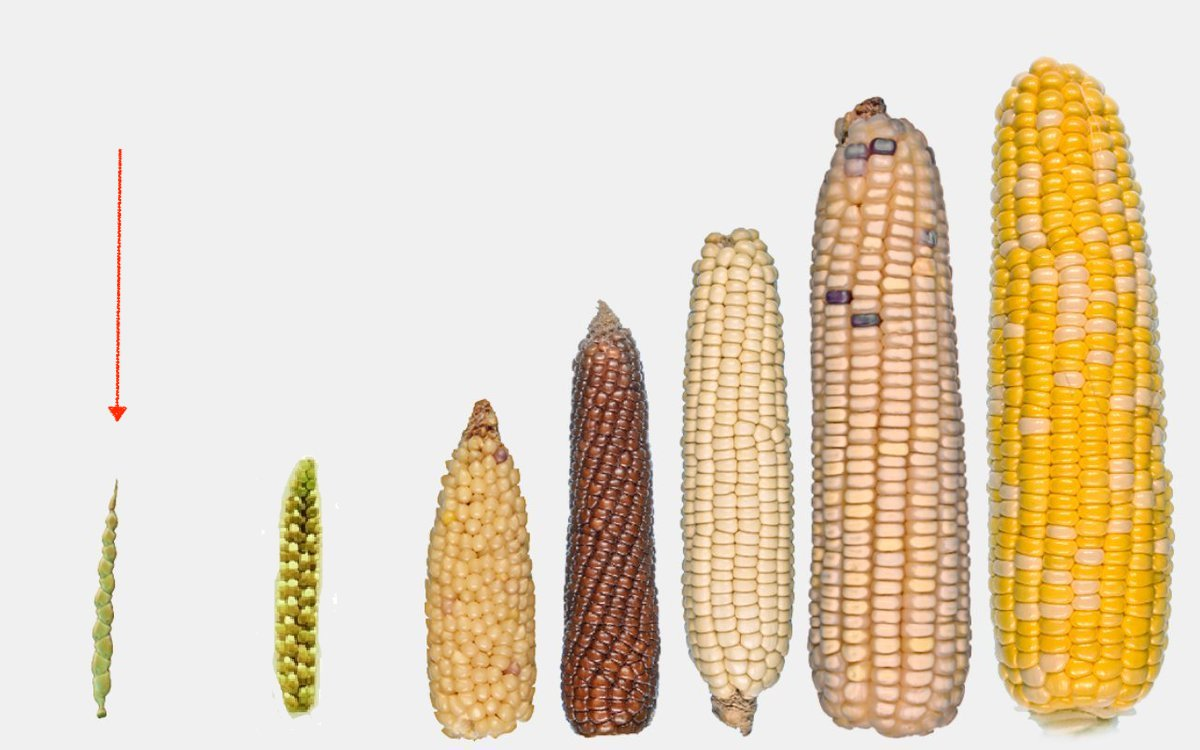
\includegraphics[width=0.9\linewidth]{./../images/maize_breeding} \caption{Evolutionary history of maize}\label{fig:maize-domestication}
\end{figure}

\end{columns}
\end{frame}

\begin{frame}{}
\protect\hypertarget{section}{}
\begin{columns}{}
  \column{0.45\textwidth}
  \begin{itemize}
  \footnotesize
  \item Domestication scars are typically vertically asymmetric rather than round, deeply recessed rather than flat, and often have wide and irregular or elongate holes where the vasculature has torn
  \item Specimens from wild populations do not show these features
  \item Domesticated-type attachments are typical of later archaeological rice spikelet bases.
  \end{itemize}

  \column{0.55\textwidth}

\begin{figure}
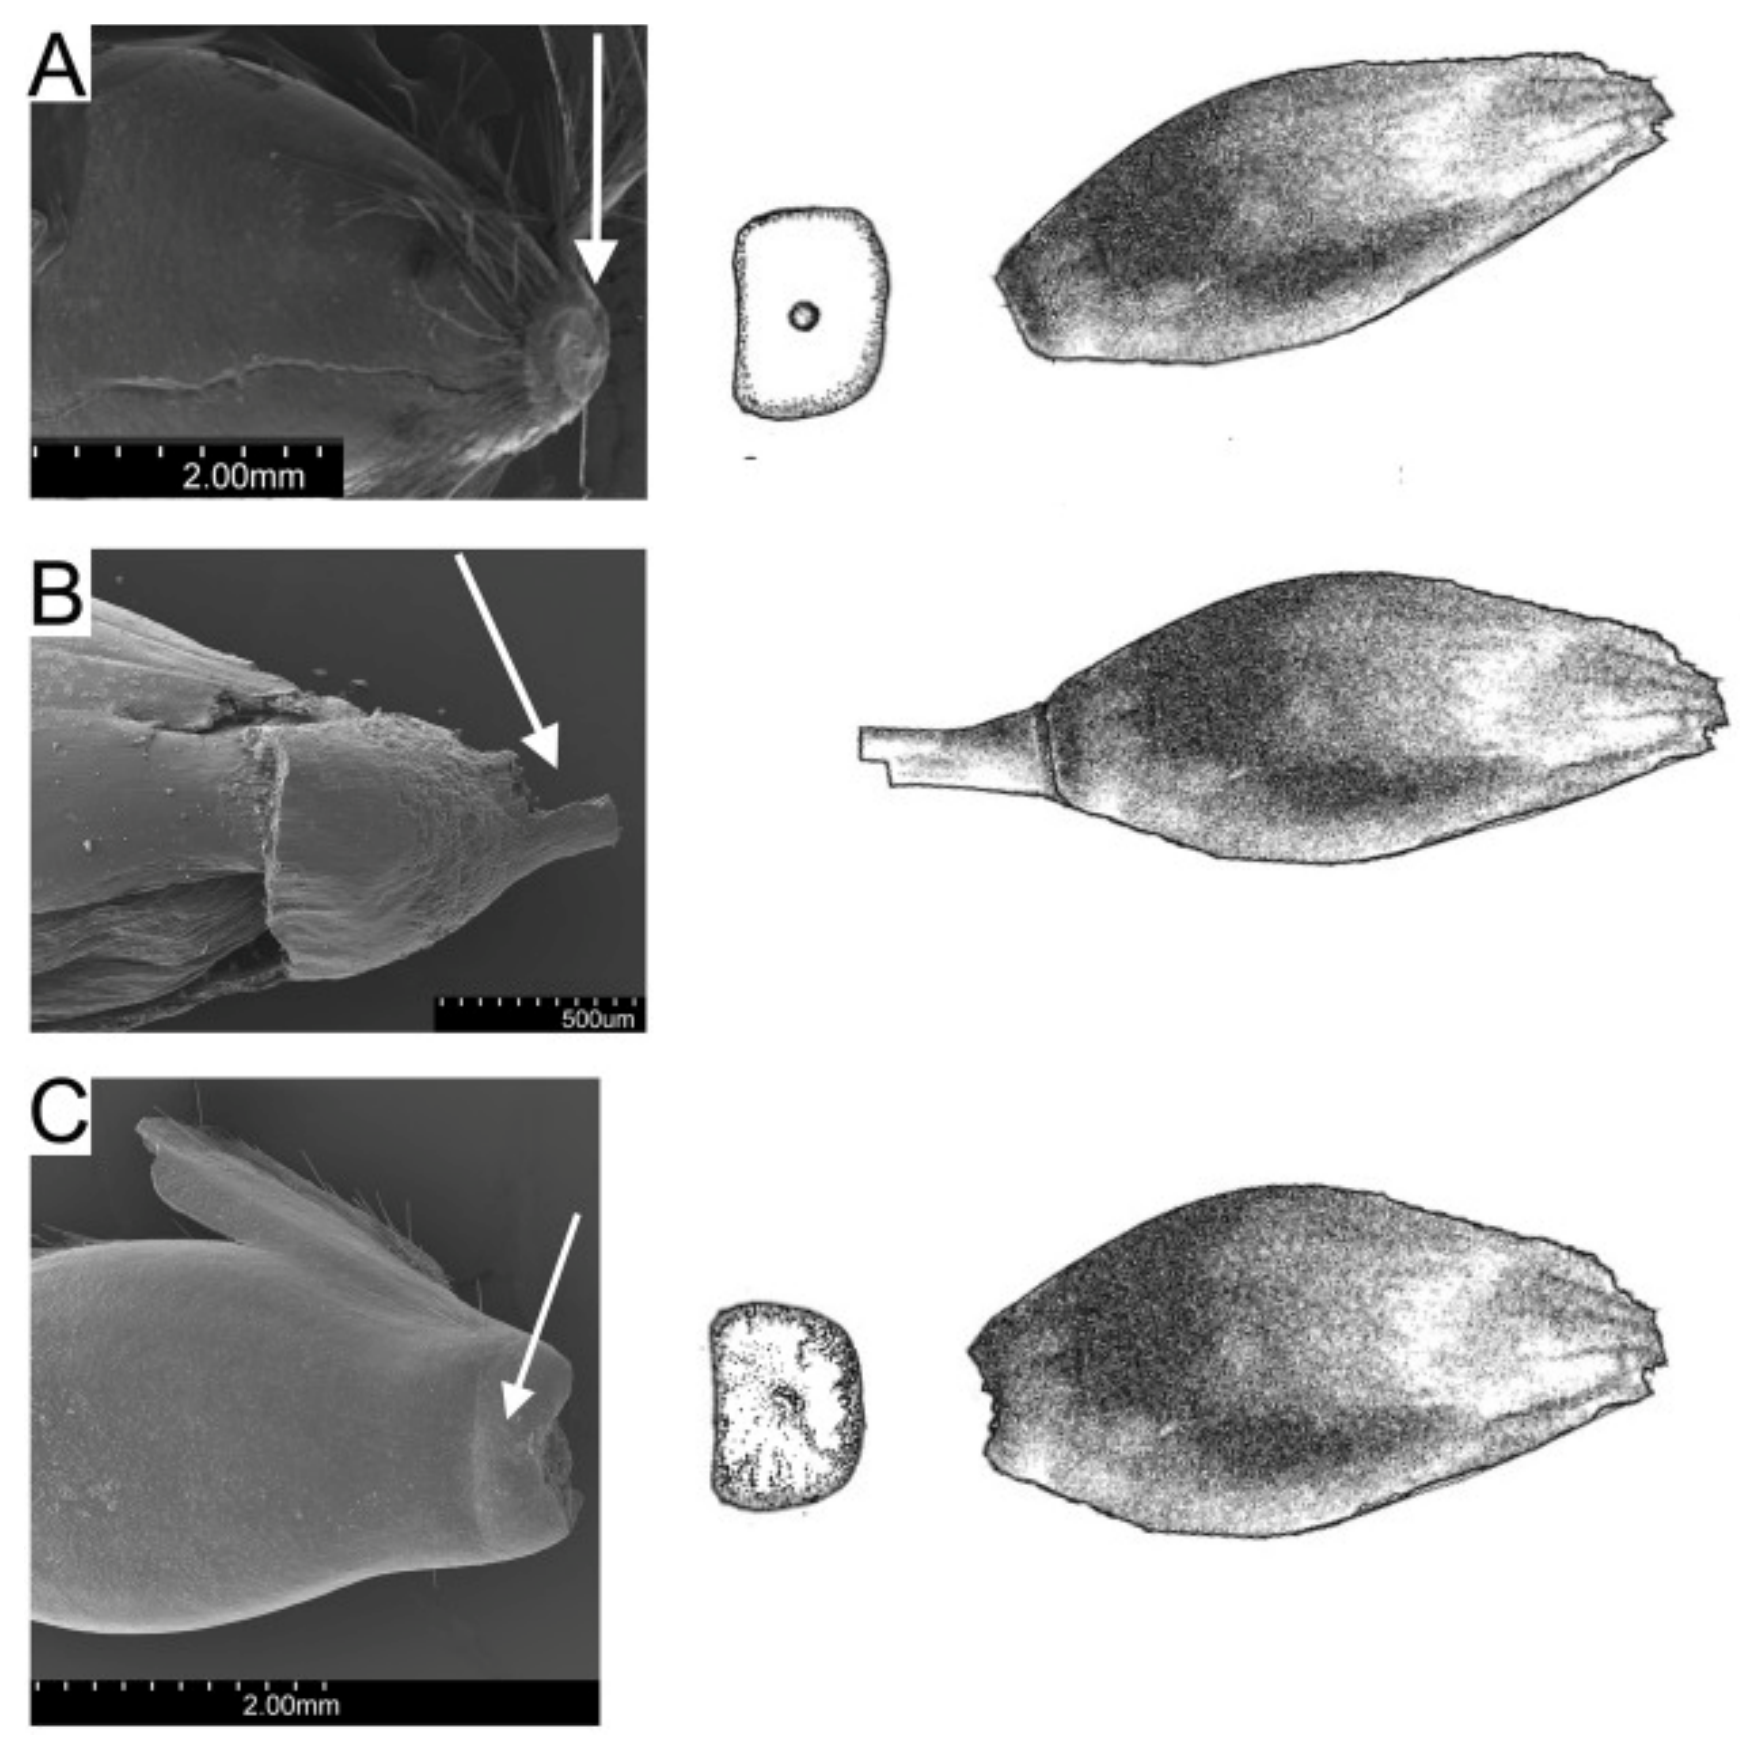
\includegraphics[width=0.65\linewidth]{../images/comparative-sem-spikelet-scar-types} \caption{Comparative SEM (left) and hand illustrated (right) images of reference specimens showing: A-smooth scar in wild-type; B-torn rachillas (30-100\%) in domesticates and immature (green-harvested) wilds; C-'rip scar' (upto 70\% in domesticates).}\label{fig:domesticated-wild-spikelet-base}
\end{figure}

\end{columns}

\footnotesize

\begin{itemize}
\tightlist
\item
  Refer to Fuller et al. (2009), Wu et al. (2017) for detailed
  pre-historic dating based accounts of rice domestication.
\item
  Figure \ref{fig:domesticated-wild-spikelet-base} shows characteristic
  domestication syndrome for spikelet base-rachis interaction in
  domesticated versus wild Sorghum crop. (For complete account refer to
  Barron et al. (2020).)
\end{itemize}
\end{frame}

\begin{frame}{}
\protect\hypertarget{section-1}{}
\begin{itemize}
\tightlist
\item
  Because of the roles of humans, the process results characteristics
  that are beneficial to humans but some that would be disadvantageous
  for plants in their natural habitats.
\item
  Results are the plants that are adapted to supervised cultural
  conditions and which posses characteristics that are preferred by
  producers and consumers.
\item
  E.g. Modern corn stripped is completely of its seed dispersal ability.
\item
  Both wild and domesticated populations are subject to evolution
\item
  Forces of selection determine what will be domesticated and that which
  will continue in wild

  \begin{itemize}
  \tightlist
  \item
    The natural selection favours plant phenotypes which have the
    greatest chance of survival, reproduction, and distribution of
    progeny.
  \item
    Human selection is the result of conscious decisions by a farmer or
    plant breeder to keep the progeny of a particular parent and discard
    others.
  \end{itemize}
\end{itemize}
\end{frame}

\begin{frame}{}
\protect\hypertarget{section-2}{}
\footnotesize

\begin{enumerate}[<+->]
\tightlist
\item
  \alert{Why did agriculture originate where it did ?}
\end{enumerate}

\begin{itemize}[<+->]
\tightlist
\item
  Domestication in different centers of origin took place roughly some
  10,000 years ago.
\item
  Hunting-gathering to agriculture transition was not an event, but a
  long process.
\item
  Because domestication syndrome is well defined, it might have taken
  lesser time to domesticate (decades/few centuries).
\item
  With few exceptions (North America and Central Asia), most
  domestication centers are located in subtropical or tropical regions
  within \(30^\circ\) latitude.
\item
  Centers of domestication are located disproportionately frequently in
  biodiversity hotspots.
\item
  Why other regions with similar geographic and eco-climatic
  characteristics did not become centers of domestication?

  \begin{itemize}[<+->]
  \tightlist
  \item
    Some cultures were only known to manipulate vegetation without
    actually turning to full-fledged agriculture
  \end{itemize}
\end{itemize}
\end{frame}

\begin{frame}{}
\protect\hypertarget{section-3}{}
\footnotesize

\begin{enumerate}[<+->]
\setcounter{enumi}{1}
\tightlist
\item
  \alert{What is the pattern of domestication for crops and animals?}
\end{enumerate}

\begin{itemize}[<+->]
\tightlist
\item
  The number and location of domestication of a crop also defines
  overall genetic diversity.
\item
  A crop may have a single or multiple domestications.
\item
  Traditionally, the origin of domestication of a crop has been
  determined based on the geographic distribution of the wild ancestor,
  complemented when possible with archaeological remains. Evidence from:

  \begin{itemize}[<+->]
  \tightlist
  \item
    earlier: floation technique
  \item
    recent: molecular genetics
  \end{itemize}
\end{itemize}
\end{frame}

\begin{frame}{}
\protect\hypertarget{section-4}{}
\footnotesize

\begin{enumerate}[<+->]
\setcounter{enumi}{2}
\tightlist
\item
  \alert{How did agricultural ecosystems develop ?}
\end{enumerate}

\begin{itemize}[<+->]
\tightlist
\item
  Genetic studies have focused on individual crop and animal species.
  Yet, the sum of just these components do not define agriculture to
  full extent.
\item
  Agriculture includes agronomic and nutritional complementary systems

  \begin{itemize}[<+->]
  \tightlist
  \item
    Most center of domestication include a combination of protein
    (legume) and starch (cereal/root) staple
  \end{itemize}
\item
  Compared to hunting and gathering, agriculture maximized the chances
  of obtaining food per unit land. That led to development of
  agriculturally based societies.
\item
  With expansion of agriculture, its ecological footprint increased,
  thus the need for sustainable agriculture that maintains its resource
  basis.
\item
  In turn, agriculture could potentially start exerting selection
  pressures that affect human phenotypes -- resistance to malaria,
  starch consumption, and lactose intolerance
\end{itemize}

\begin{enumerate}[<+->]
\setcounter{enumi}{3}
\tightlist
\item
  \alert{How did agricultural ecosystems spread from the centers of origin?}
\end{enumerate}

\begin{itemize}[<+->]
\tightlist
\item
  Two, non-mutually exclusive, modes of dispersal have been proposed to
  account for the spread of agriculture.

  \begin{enumerate}[<+->]
  \tightlist
  \item
    Culturally dispersion through adoption by non-migrating populations.
  \item
    Migration of population from center of domestication
  \end{enumerate}
\end{itemize}
\end{frame}

\begin{frame}{Weed}
\protect\hypertarget{weed}{}
\begin{itemize}
\tightlist
\item
  ``A plant in the wrong place''
\item
  How accurate is the definition ?
\item
  We define weeds as plants we do not want that compete for resources
  with those we do want.
\item
  Clearly we have criteria about which plants we want and those that
  fail those criteria.
\item
  In evolutionary terms, it is the cultivated plants that are ``fitter''
  than the weeds, as they have characteristics which we want, and since
  in the fi eld and the garden we have largely substituted ourselves for
  nature, and here it is us who control the evolutionary process.
\item
  However, many commercially grown plants survive as volunteer weeds, or
  ``escapes'', in either the same, or different, regions to those in
  which they are most commonly grown commercially.
\end{itemize}
\end{frame}

\begin{frame}{}
\protect\hypertarget{section-5}{}
\begin{figure}

{\centering 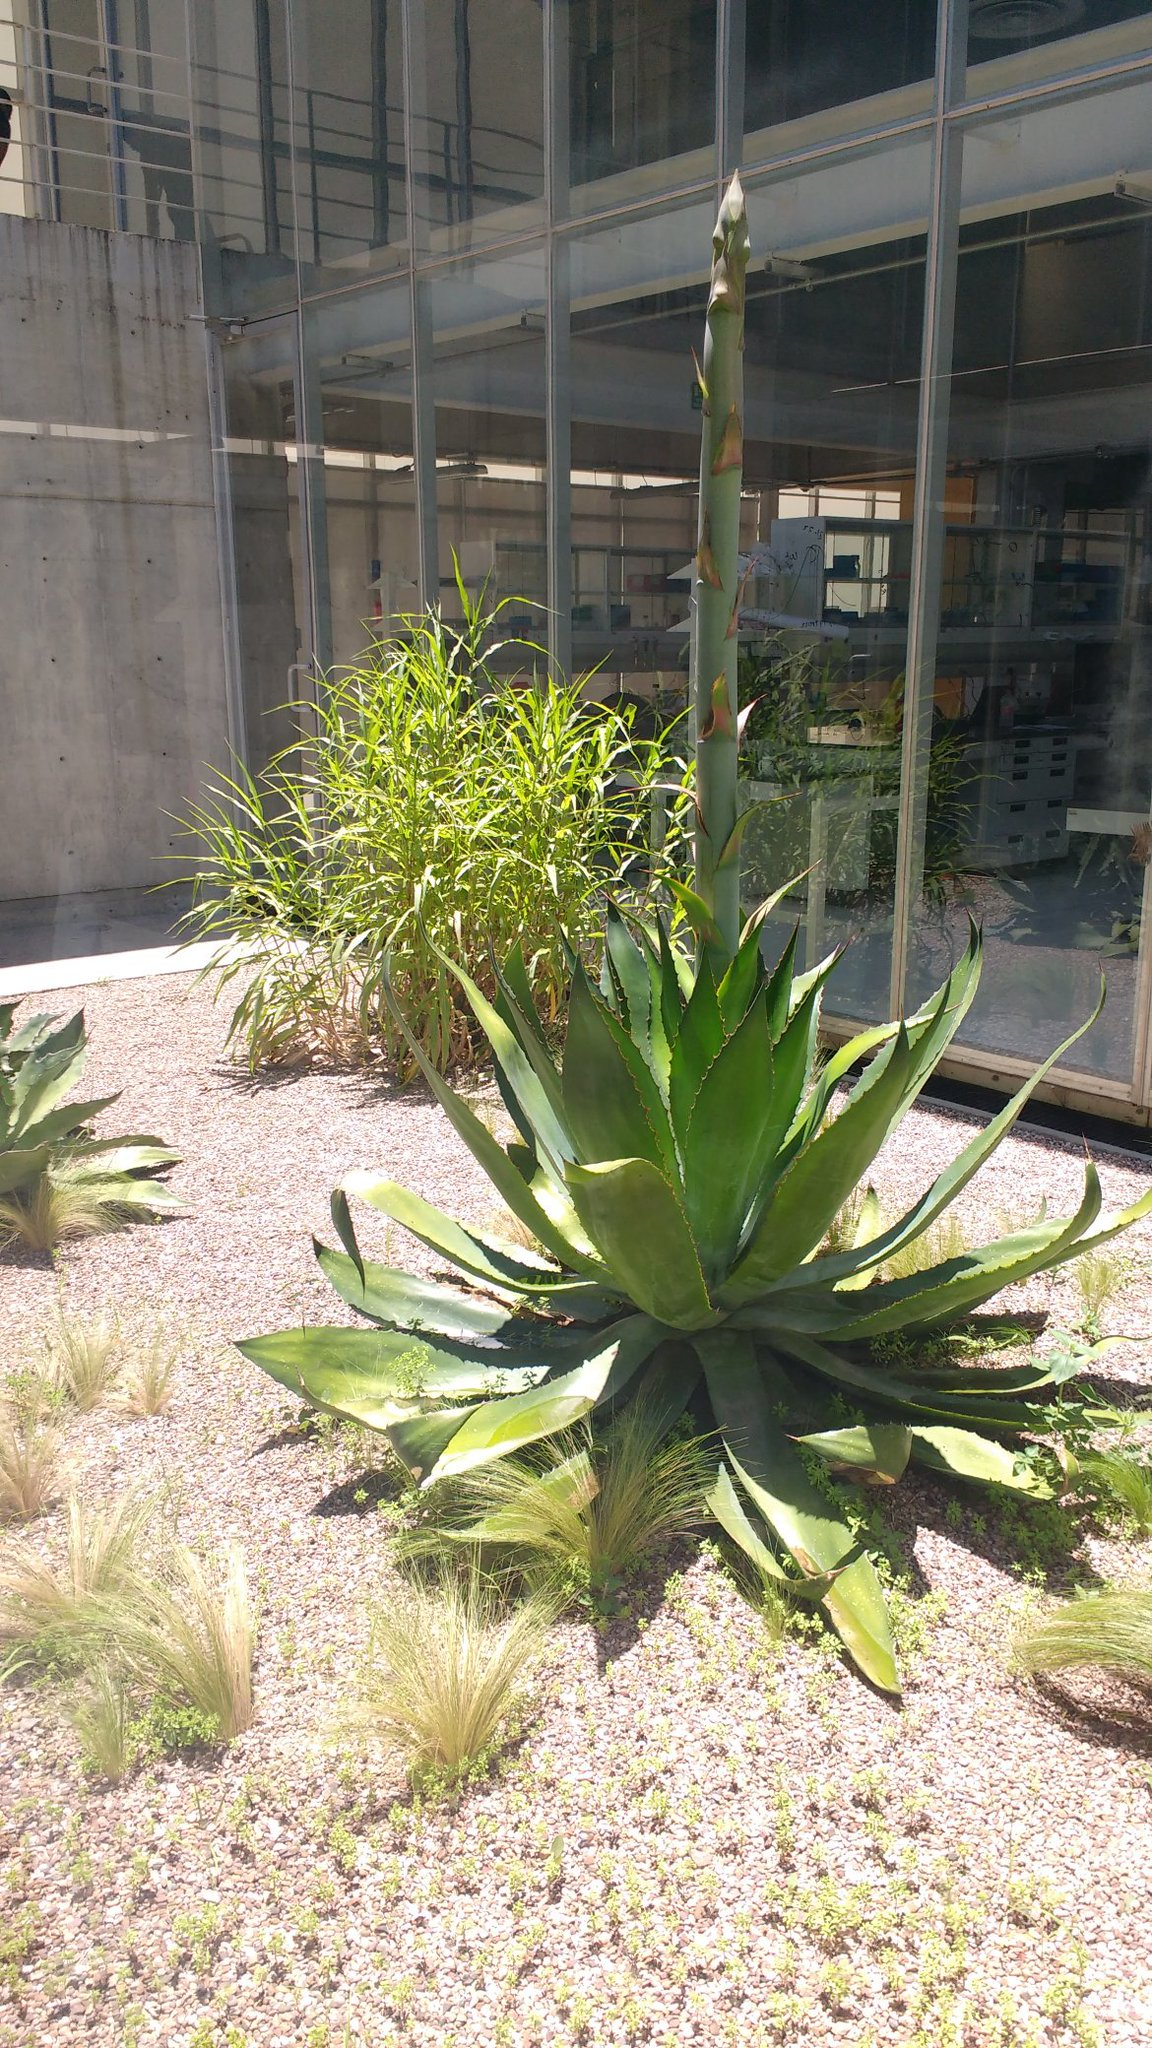
\includegraphics[width=0.26\linewidth]{./../images/Perennial_teosinte} 

}

\caption{Perennial teosinte}\label{fig:weed-vs-crop}
\end{figure}
\end{frame}

\hypertarget{domestication-syndrome-changes-in-plant-species-under-domestication}{%
\subsection{Domestication syndrome (Changes in plant species under
domestication)}\label{domestication-syndrome-changes-in-plant-species-under-domestication}}

\begin{frame}{}
\protect\hypertarget{section-6}{}
\begin{table}

\caption{\label{tab:domestication-syndrome}Changes in plants under domestication}
\centering
\fontsize{6}{8}\selectfont
\begin{tabular}[t]{>{\raggedright\arraybackslash}p{16em}>{\raggedright\arraybackslash}p{40em}}
\toprule
General effect & Specific traits altered\\
\midrule
\textbf{\cellcolor{gray!6}{Increased seedling vigor (more plants germinating)}} & \cellcolor{gray!6}{Loss of seed or tuber dormancy}\\
\textbf{} & Large seeds\\
\textbf{\cellcolor{gray!6}{Modified reproductive system}} & \cellcolor{gray!6}{Increased selfing}\\
\textbf{} & Reduced complexity of reproductive organs\\
\textbf{\cellcolor{gray!6}{}} & \cellcolor{gray!6}{Vegetatively reproducing plants}\\
\addlinespace
\textbf{} & Altered photoperiod sensitivity\\
\textbf{\cellcolor{gray!6}{}} & \cellcolor{gray!6}{Shift in sex form of species}\\
\textbf{} & Promotion of asexual reproduction\\
\textbf{\cellcolor{gray!6}{Increased number of seeds harvested}} & \cellcolor{gray!6}{Non-shattering}\\
\textbf{} & Reduced number of branches (more fruits per branch)\\
\bottomrule
\end{tabular}
\end{table}
\end{frame}

\begin{frame}{}
\protect\hypertarget{section-7}{}
\begin{table}

\caption{\label{tab:domestication-syndrome2}Changes in plants under domestication (...continued)}
\centering
\fontsize{6}{8}\selectfont
\begin{tabular}[t]{>{\raggedright\arraybackslash}p{16em}>{\raggedright\arraybackslash}p{40em}}
\toprule
General effect & Specific traits altered\\
\midrule
\textbf{\cellcolor{gray!6}{Increased appeal to consumers}} & \cellcolor{gray!6}{Attractive fruit/seed colors and patterns}\\
\textbf{} & Enhanced flavor, texture, and taste of seeds/fruits/tubers (food parts)\\
\textbf{\cellcolor{gray!6}{}} & \cellcolor{gray!6}{Reduced toxic principles (safer food)}\\
\textbf{} & Larger fruits\\
\textbf{\cellcolor{gray!6}{}} & \cellcolor{gray!6}{Reduces spikiness}\\
\addlinespace
\textbf{} & Increase in economic yield (HI)\\
\textbf{\cellcolor{gray!6}{Altered plant architecture and growth habit}} & \cellcolor{gray!6}{Compact growth habit (Determinacy, reduced plant size, dwarfism)}\\
\textbf{} & Reduced branching\\
\textbf{\cellcolor{gray!6}{}} & \cellcolor{gray!6}{Decreases in variability within a variety}\\
\textbf{Change in developmental phenology} & Change in life cycle (normally from perennial to annual for seed crops, and from annual to biennial for vegetable crops)\\
\bottomrule
\end{tabular}
\end{table}
\end{frame}

\begin{frame}{Wild versus domestication traits}
\protect\hypertarget{wild-versus-domestication-traits}{}
\begin{columns}[T,onlytextwidth]
  
  \column{0.5\textwidth}
  
\begin{figure}
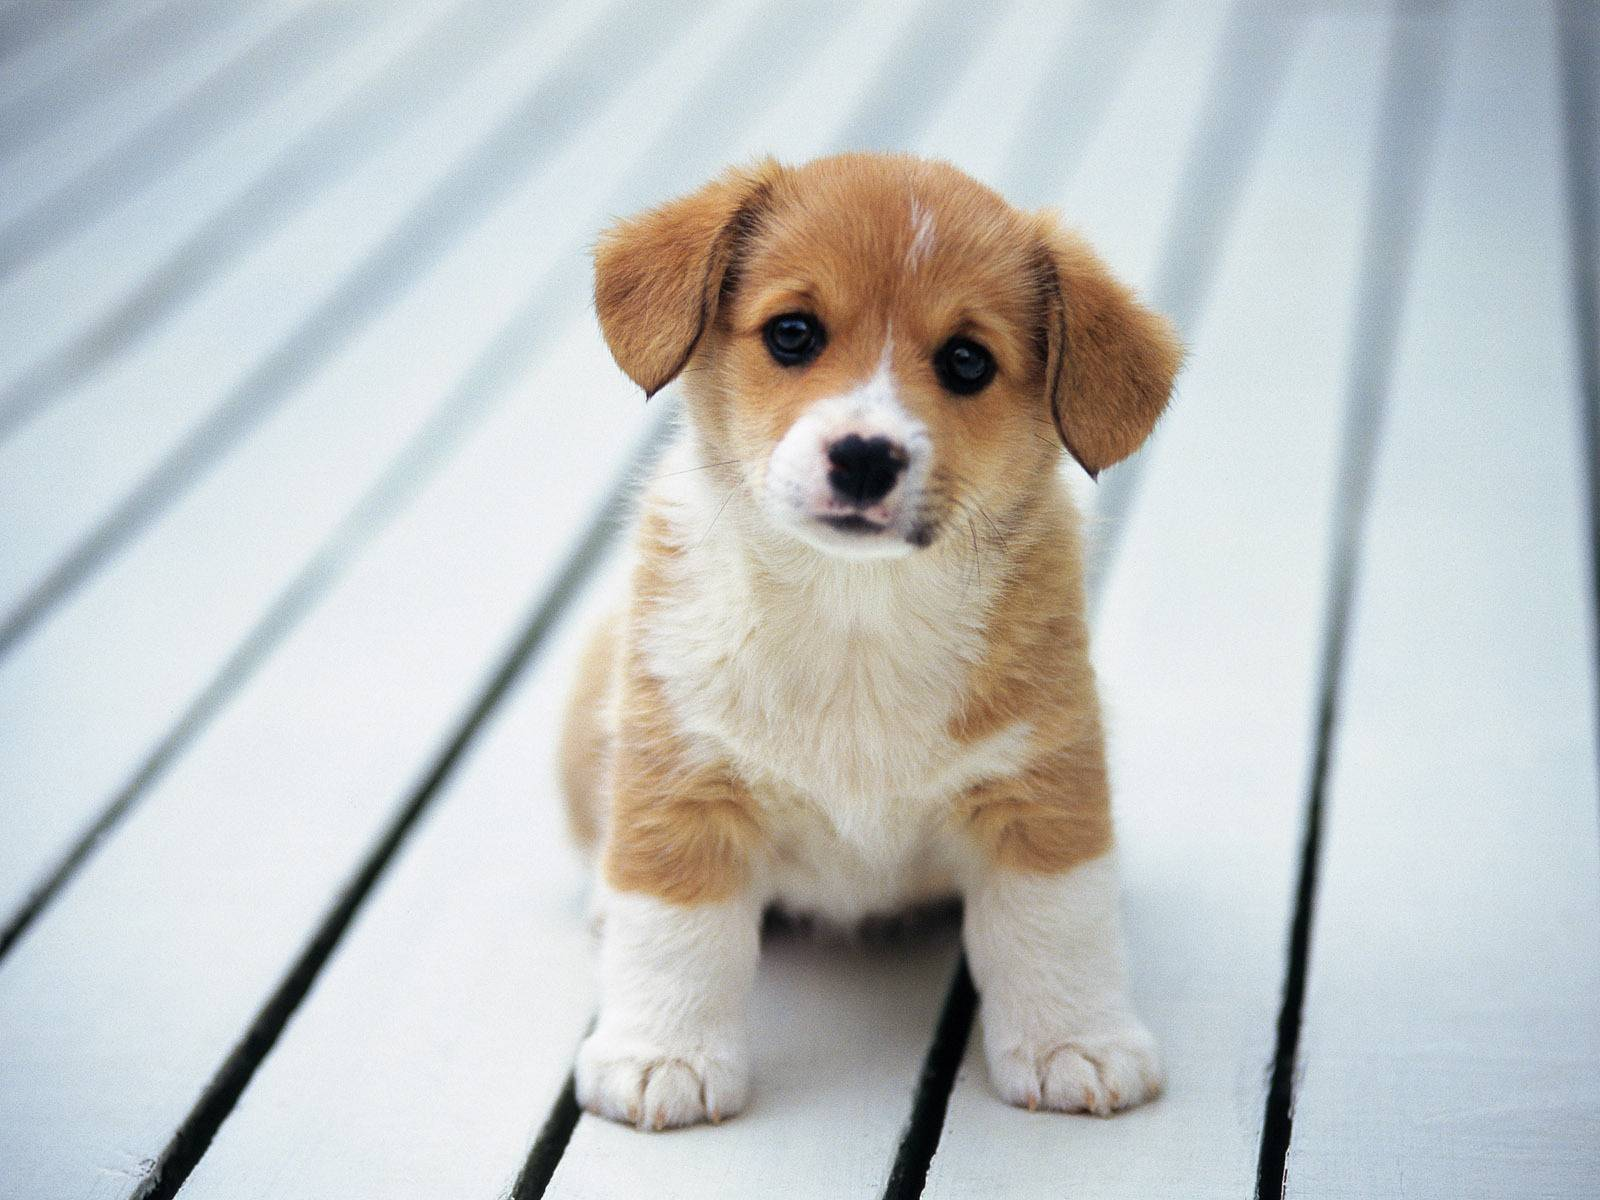
\includegraphics[width=0.8\linewidth]{./../images/domestic_dog_puppy} \caption{Domesticated dog}\label{fig:domesticated}
\end{figure}

  \column{0.5\textwidth}

\begin{figure}
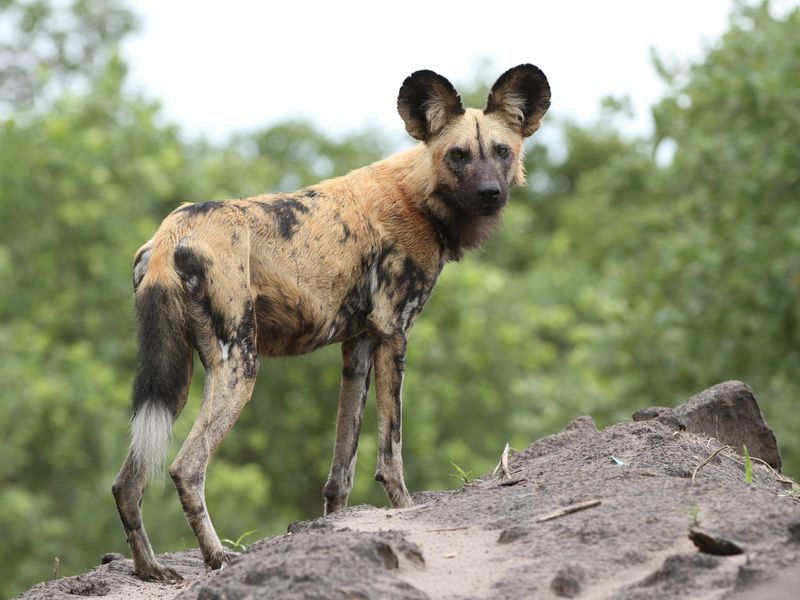
\includegraphics[width=0.8\linewidth]{./../images/wild_dog_african} \caption{Wild dog}\label{fig:wild}
\end{figure}

\end{columns}
\end{frame}

\begin{frame}{Wild verus domestication traits (context)}
\protect\hypertarget{wild-verus-domestication-traits-context}{}
\begin{itemize}
\item
  Wild cereal plants tend to have many small seeds at maturity and
  disperse their seed by shattering. These seeds also are likely to be
  attached to a strong awn to aid dispersal.
\item
  Similarly, wild potato species produce many small tubers, have their
  tubers develop at the end of very long stolons (so that daughter
  plants do not have to occupy ground too close to the parent), and many
  have tubers with high levels of toxin, which discourage animals from
  eating them.
\item
  Breeders have developed cereal cultivars which have fewer, but larger
  seeds, that do not shatter their seeds at maturity and that have a
  non-persistent awn.
\end{itemize}
\end{frame}

\begin{frame}{}
\protect\hypertarget{section-8}{}
\begin{itemize}
\item
  Similarly potato breeders have selected plants with fewer, but larger
  tubers, shorter stolons and with reduced levels of toxins in the
  tuber.
\item
  Human selection also has produced crops that are more uniform in the
  expression of many of their characteristics. For example, they have
  selected seeds that all mature at the same time, with uniform
  germination, and fruits with uniform fruit size and shape.
\item
  In more recent times plant breeders' selection has tended to result in
  shorter plants, greater harvest index, and increased ease of harvest
  (especially mechanized).
\end{itemize}
\end{frame}

\begin{frame}{}
\protect\hypertarget{section-9}{}
\begin{figure}

{\centering 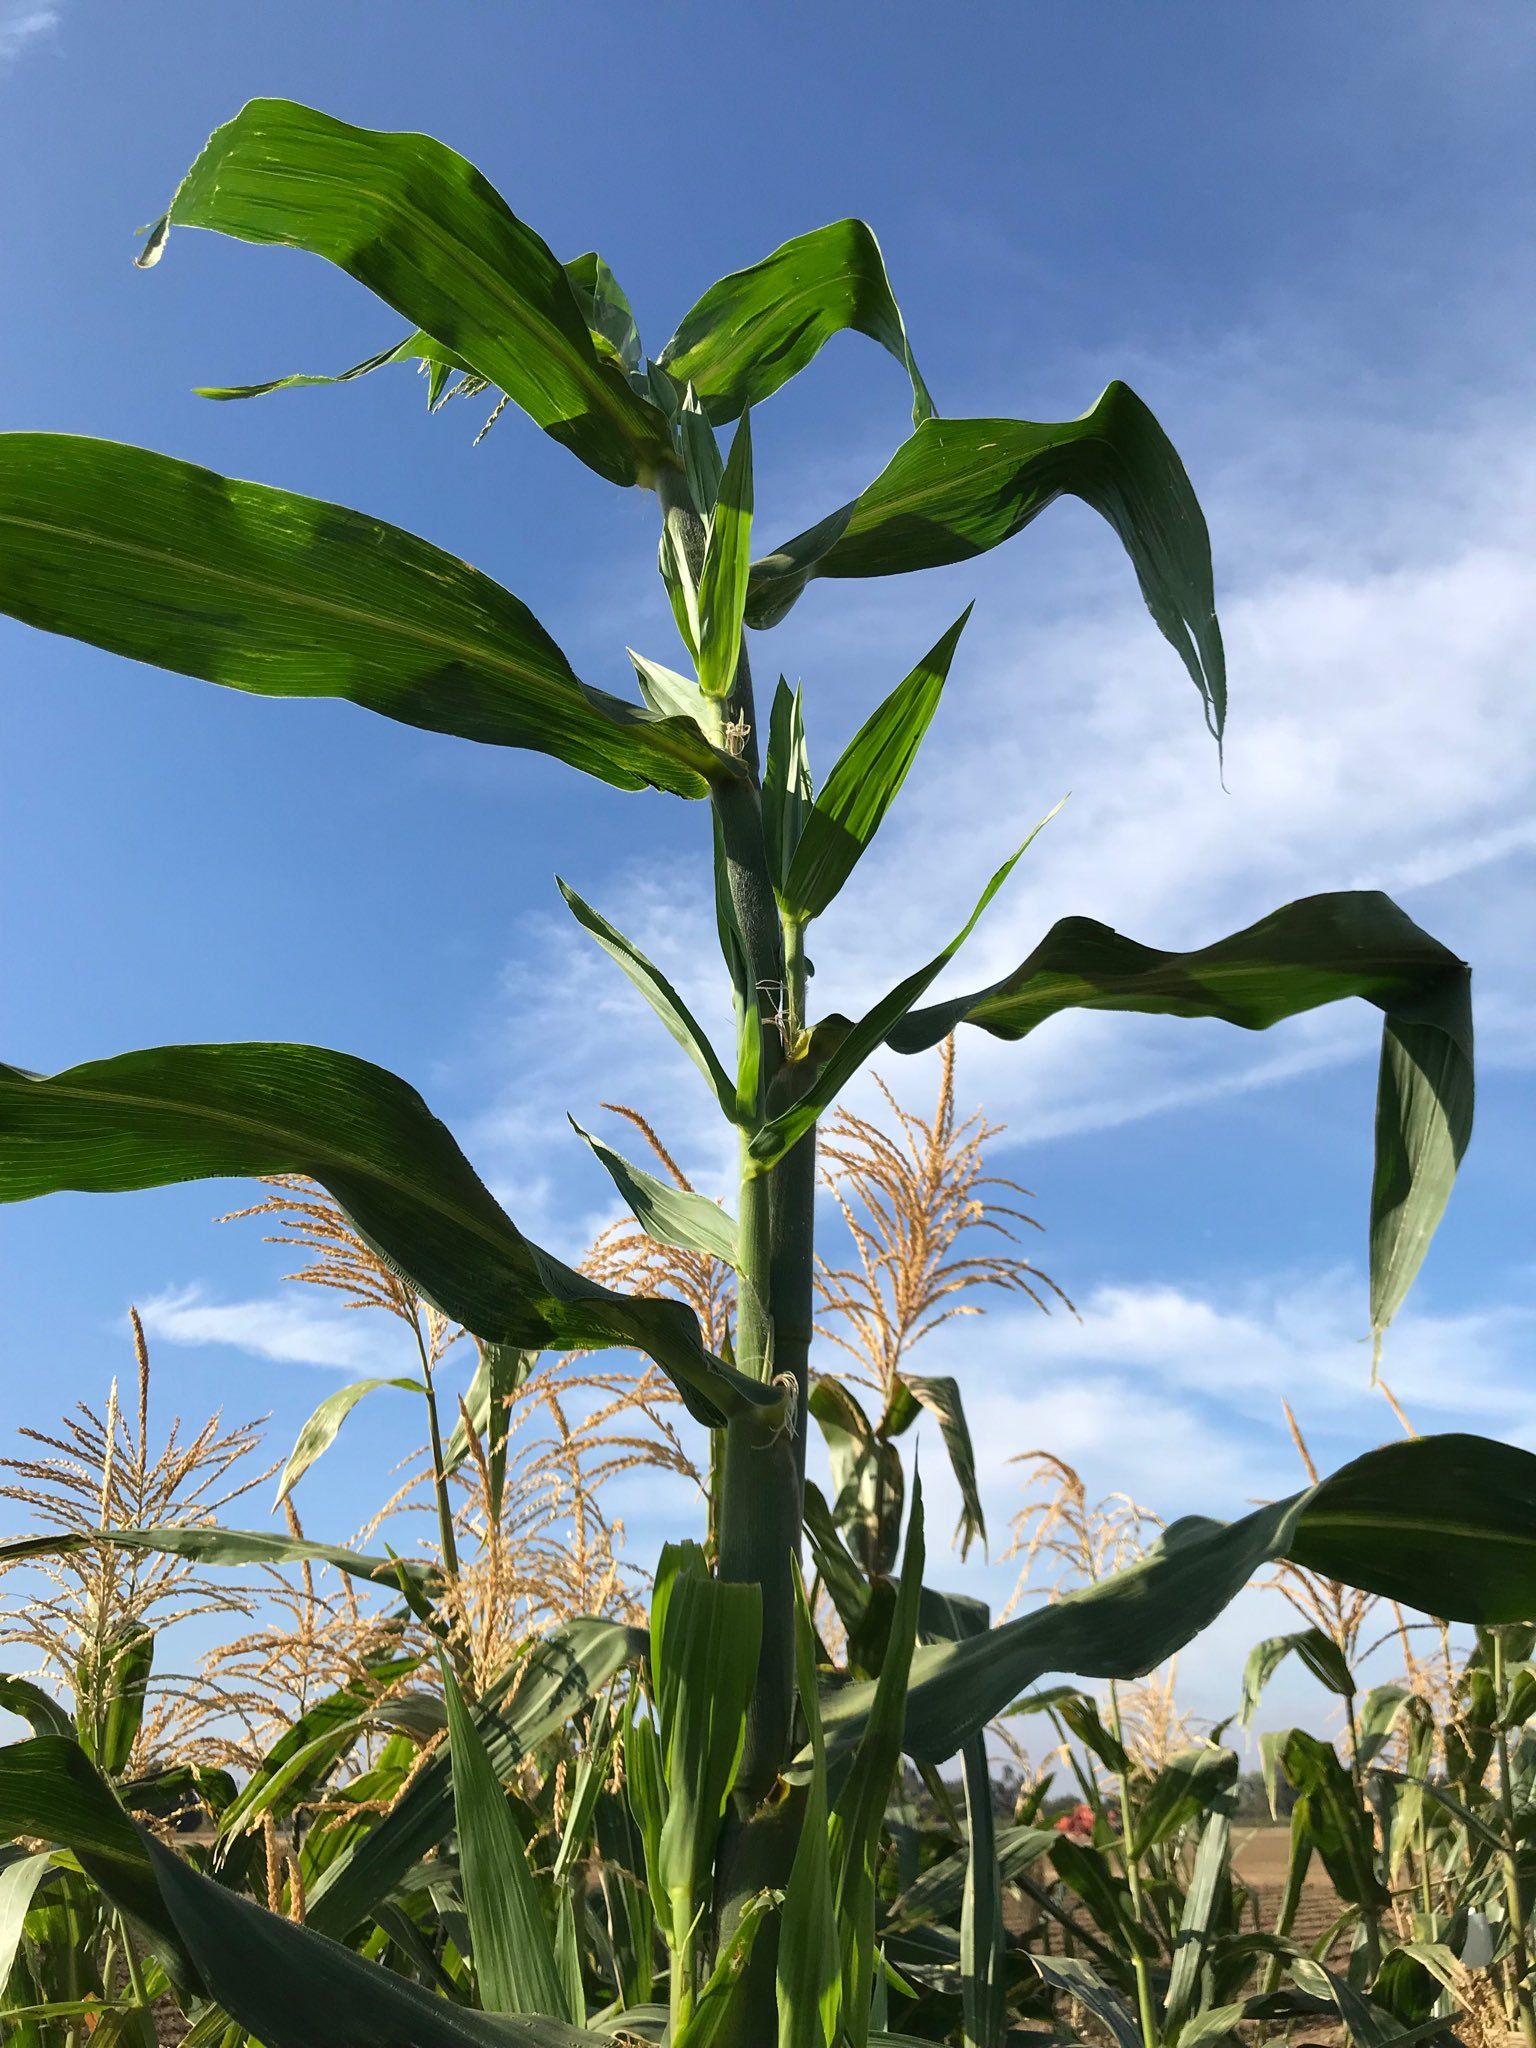
\includegraphics[width=0.4\linewidth]{./../images/Teosinte_maize_hybrid_cross} 

}

\caption{Teosinte maize hybrid}\label{fig:unnamed-chunk-1}
\end{figure}
\end{frame}

\hypertarget{origin-and-diversity}{%
\section{Origin and diversity}\label{origin-and-diversity}}

\hypertarget{gene-pool}{%
\subsection{Gene pool}\label{gene-pool}}

\begin{frame}{Germplasm and gene pool concept}
\protect\hypertarget{germplasm-and-gene-pool-concept}{}
\footnotesize

\begin{itemize}
\tightlist
\item
  Germplasm refers to the genetic material that can be used to
  perpetuate a species or population
\item
  Provides the material to initiate a breeding program
\item
  Sometimes only germplasm screening and evaluation is practiced for
  introduction of improved variety in a region
\item
  Certain institutional sets-ups such as gene banks are charged with the
  responsibility of assembling, cataloguing, storing and managing large
  number of germplasm. This allows for quick retrieval.
\item
  J.R. Harlan and J.M.J. de Wet proposed a categorization of gene pools
  of cultivated germplasm according to the feasibility of gene transfer
  or gene flow from those species to the crop species.
\end{itemize}

\begin{figure}
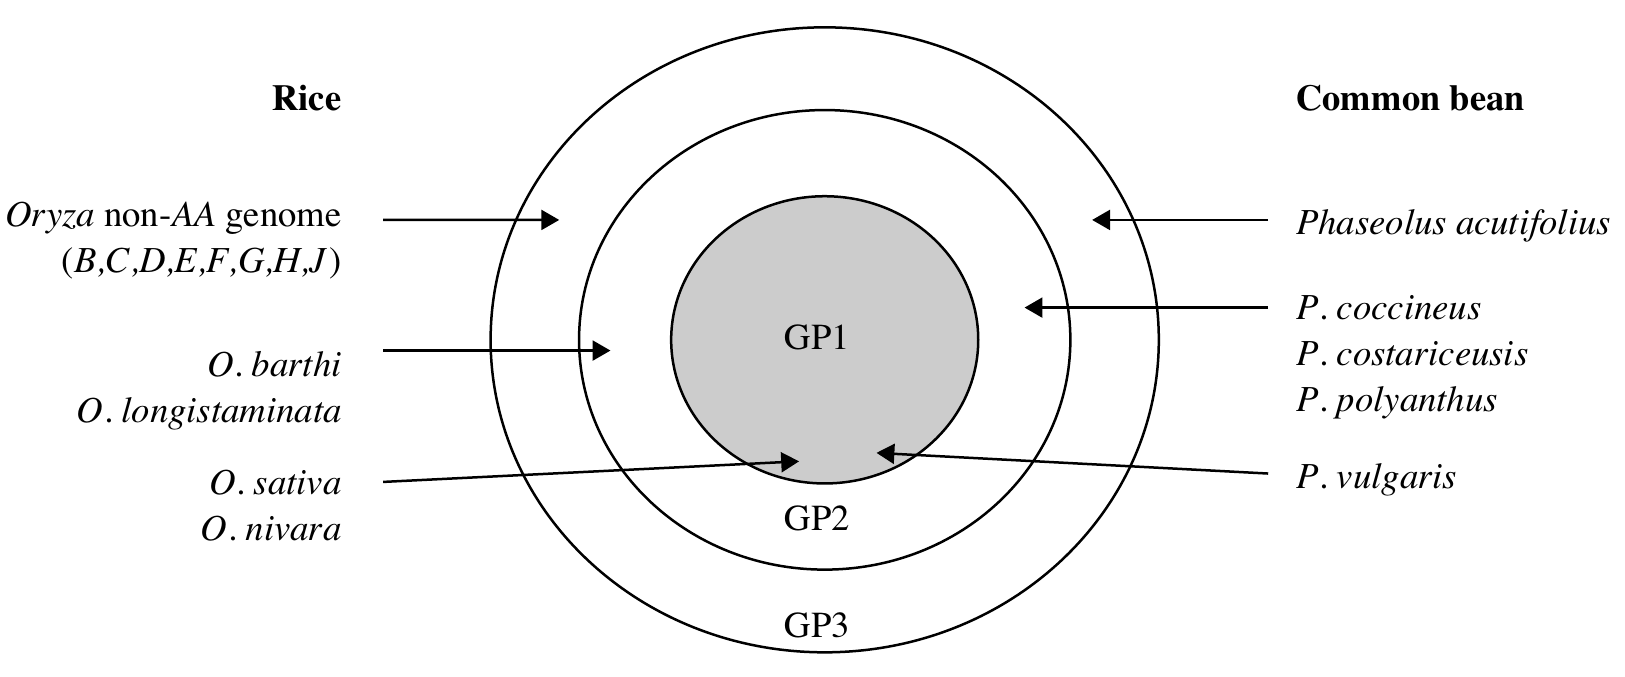
\includegraphics[width=0.42\linewidth]{./../images/crop_gene_pools} \caption{Crop gene pools; A system proposed by Harlan}\label{fig:gene-pools}
\end{figure}
\end{frame}

\begin{frame}{Types of gene pool}
\protect\hypertarget{types-of-gene-pool}{}
\begin{itemize}
\tightlist
\item
  \emph{Primary gene pool (GP1)}

  \begin{itemize}
  \tightlist
  \item
    GP1 consists of biological species that can be intercrossed easily
    (interfertile) without any problems with fertility of the progeny.
    That is, there is no restriction to gene exchange between members of
    the group. This group may contain both cultivated and wild
    progenitors of the species.
  \end{itemize}
\item
  \emph{Secondary gene pool (GP2)}

  \begin{itemize}
  \tightlist
  \item
    Members of this gene pool include both cultivated and wild relatives
    of the crop species. They are more distantly related and have
    crossability problems. Nonetheless, crossing produces hybrids and
    derivatives that are sufficiently fertile to allow gene flow. GP2
    species can cross with those in GP1, with some fertility of the F1,
    but more difficulty with success.
  \end{itemize}
\item
  \emph{Tertiary gene pool (GP3)}

  \begin{itemize}
  \tightlist
  \item
    GP3 involves the outer limits of potential genetic resources. Gene
    transfer by hybridization between GP1 and GP3 is very problematic,
    resulting in lethality, sterility, and other abnormalities. To
    exploit germplasm from distant relatives, tools such as embryo
    rescue and bridge crossing may be used to nurture an embryo from a
    wide cross to a full plant and to obtain fertile plants.
  \end{itemize}
\end{itemize}
\end{frame}

\hypertarget{the-vavilov-concept}{%
\subsection{The Vavilov Concept}\label{the-vavilov-concept}}

\begin{frame}{}
\protect\hypertarget{section-10}{}
\begin{itemize}
\tightlist
\item
  Nikolai I. Vavilov (1887-1942), the Russian botanist and plant
  breeder, demonstrated the existence of `centres of origin' of
  cultivated plants (more correctly named today as `centres of
  diversity'), in which can be found the highest level of genetic
  variability of a species. This variability, which arises in nature by
  mutation spontaneous hybridization, introgression and changes in
  chromosome form and number, provides the means by which adaptation to
  heterogenous environments can occur.
\item
  It allows the breeder to identify sources of variation for specific
  characteristics. The extension of this principle to related species
  was formulated by Vavilov in his `law of homologous series of
  variation'. This law allows the prediction of the appearance of a
  given type of mutation in a plant species when such a type has been
  found in another species phylogenetically related to the first.
\item
  Defined plant breeding as `plant evolution directed by man'; concept
  of `applied plant genetics'.
\end{itemize}
\end{frame}

\hypertarget{center-of-origin-and-center-of-diversity}{%
\subsection{Center of origin and center of
diversity}\label{center-of-origin-and-center-of-diversity}}

\begin{frame}{}
\protect\hypertarget{section-11}{}
\begin{itemize}
\tightlist
\item
  CBD takes the ``centre of origin'' and the ``centre of crop
  diversity'' as references referring to the scientific rather than
  political connecting points for the definition of
  origin\footnote<.->{Refer to Rights to plant genetic resources and
    traditional knowledge}.
\item
  It defines ``centre of origin'' as ``a geographical area where a plant
  species, either domesticated or wild, first developed its distinctive
  properties'', and ``centre of crop diversity'' as ``the geographic
  area containing a high level of genetic diversity for crop species in
  in-situ conditions'' (Articles 2.8 and 2.9).
\item
  On the basis of soveignty of states over their natural resources,
  ``the country of origin of genetic resources'' is defined as the
  country that possesses the genetic resources in \emph{in situ}
  conditions (Article 2.4).
\end{itemize}
\end{frame}

\hypertarget{domestication-and-origin-of-major-crop-species}{%
\subsection{Domestication and origin of major crop
species}\label{domestication-and-origin-of-major-crop-species}}

\begin{frame}{}
\protect\hypertarget{section-12}{}
\begin{table}

\caption{\label{tab:domestication-origin}Estimated time of domestication and centre of origin of major crop species; @brown2014plant, Page 23}
\centering
\fontsize{6}{8}\selectfont
\begin{tabular}[t]{>{\raggedright\arraybackslash}p{8em}>{\raggedright\arraybackslash}p{12em}>{\raggedright\arraybackslash}p{8em}>{\raggedright\arraybackslash}p{12em}}
\toprule
Crop category & Crop & Length of time domesticated (years) & Possible region of origin\\
\midrule
\textbf{\cellcolor{gray!6}{Cereals}} & \cellcolor{gray!6}{Maize, Zea mays} & \cellcolor{gray!6}{7000} & \cellcolor{gray!6}{Mexico, Central America}\\
\textbf{Cereals} & Rice, Oryza sativa & 4500 & Thailand, Southern China\\
\textbf{\cellcolor{gray!6}{Cereals}} & \cellcolor{gray!6}{Wheat, Triticum spp.} & \cellcolor{gray!6}{8500} & \cellcolor{gray!6}{Syria, Jordan, Israel, Iraq}\\
\textbf{Cereals} & Barley, Hordeum vulgare & 9000 & Syria, Jordan, Israel, Iraq\\
\textbf{\cellcolor{gray!6}{Cereals}} & \cellcolor{gray!6}{Sorghum, Sorghum bicolor} & \cellcolor{gray!6}{8000} & \cellcolor{gray!6}{Equatorial Africa}\\
\addlinespace
\textbf{Oilseeds} & Soybean, Glycine max & 2000 & North China\\
\textbf{\cellcolor{gray!6}{Oilseeds}} & \cellcolor{gray!6}{Oil palm, Elaeis guineensis} & \cellcolor{gray!6}{9000} & \cellcolor{gray!6}{Central Africa}\\
\textbf{Oilseeds} & Coconut palm, Cocos nucifera & 100 & Southern Asia\\
\textbf{\cellcolor{gray!6}{Oilseeds}} & \cellcolor{gray!6}{Rapeseed, Brassica napus} & \cellcolor{gray!6}{500} & \cellcolor{gray!6}{Mediterranean Europe}\\
\textbf{Oilseeds} & Sunflower, Helianthus annus & 3000 & Western United States\\
\addlinespace
\textbf{\cellcolor{gray!6}{Pulses}} & \cellcolor{gray!6}{Beans, Phaseolus spp} & \cellcolor{gray!6}{7000} & \cellcolor{gray!6}{Centra America, Mexico}\\
\textbf{Pulses} & Lentil, Lens culinaris & 7000 & Syria, Jordan, Israel, Iraq\\
\textbf{\cellcolor{gray!6}{Pulses}} & \cellcolor{gray!6}{Peas, Pisum sativum} & \cellcolor{gray!6}{9000} & \cellcolor{gray!6}{Syria, Jordan, Israel, Iraq}\\
\textbf{Root crops} & Potato, Solanum tuberosum & 7000 & Peru\\
\textbf{\cellcolor{gray!6}{Root crops}} & \cellcolor{gray!6}{Cassava, Manihot esculenta} & \cellcolor{gray!6}{5000} & \cellcolor{gray!6}{Brazil, Mexico}\\
\bottomrule
\end{tabular}
\end{table}
\end{frame}

\begin{frame}{}
\protect\hypertarget{section-13}{}
\begin{table}

\caption{\label{tab:domestication-origin2}Estimated time of domestication and centre of origin of major crop species; @brown2014plant, Page 23 (...continued)}
\centering
\fontsize{6}{8}\selectfont
\begin{tabular}[t]{>{\raggedright\arraybackslash}p{8em}>{\raggedright\arraybackslash}p{12em}>{\raggedright\arraybackslash}p{8em}>{\raggedright\arraybackslash}p{12em}}
\toprule
Crop category & Crop & Length of time domesticated (years) & Possible region of origin\\
\midrule
\textbf{\cellcolor{gray!6}{Root crops}} & \cellcolor{gray!6}{Sweet potato, Ipomoea batatas} & \cellcolor{gray!6}{6000} & \cellcolor{gray!6}{South Central America}\\
\textbf{Root crops} & Sugar beet, Beta vulgaris & 300 & Mediterranean Europe\\
\textbf{\cellcolor{gray!6}{Vegetables}} & \cellcolor{gray!6}{Tomato, Lycopersicum esculentum} & \cellcolor{gray!6}{3000} & \cellcolor{gray!6}{Western South America}\\
\textbf{Vegetables} & Cabbage, Brassica oleracea & 3000 & Mediterranean Europe\\
\textbf{\cellcolor{gray!6}{Vegetables}} & \cellcolor{gray!6}{Onion, Allium spp.} & \cellcolor{gray!6}{4500} & \cellcolor{gray!6}{Iran, Afganistan, Pakistan}\\
\addlinespace
\textbf{Fruit} & Orange, Citrus sinensis & 9000 & South-east Asia\\
\textbf{\cellcolor{gray!6}{Fruit}} & \cellcolor{gray!6}{Apple, Malus spp.} & \cellcolor{gray!6}{3000} & \cellcolor{gray!6}{Asia Minor, Central Asia}\\
\textbf{Fruit} & Grape, Vitis spp. & 7000 & Eastern Asia\\
\textbf{\cellcolor{gray!6}{Fruit}} & \cellcolor{gray!6}{Banana, Musa acuminata, M. balbisiana} & \cellcolor{gray!6}{4500} & \cellcolor{gray!6}{South-east Asia}\\
\textbf{Others} & Cotton, Gossypium spp. & 4500 & Centra America, Brazil\\
\addlinespace
\textbf{\cellcolor{gray!6}{Others}} & \cellcolor{gray!6}{Coffee, Coffea spp.} & \cellcolor{gray!6}{500} & \cellcolor{gray!6}{West Ethiopia}\\
\textbf{Others} & Rubber, Hevea brasiliensis & 200 & Brazil, Bolivia, Paraguay\\
\textbf{\cellcolor{gray!6}{Others}} & \cellcolor{gray!6}{Alfalfa, Medicago sativa} & \cellcolor{gray!6}{4000} & \cellcolor{gray!6}{Iran, Northern Pakistan}\\
\bottomrule
\end{tabular}
\end{table}
\end{frame}

\begin{frame}{Rice}
\protect\hypertarget{rice}{}
\begin{itemize}
\tightlist
\item
  Probably originated 130 MYA (Virmani and IIyas-Ahmed, 2007)
\item
  Spread as wild grass in Gondwanaland.
\item
  Both cultivated species -- \emph{O. sativa} and \emph{O. glaberrima}
  (tropical West african rice) originated from common ancestor.
\item
  Wild progenitor of \emph{O. sativa} is common asian wild rice called
  \emph{O. rufipogon} (has perennial to annual types).
\item
  Annual types of the wild progenitor called \emph{O. nivara} resulted
  in present day asian rice.
\item
  Alternative hypotheses: two distinct subspecies of rice (
  \emph{indica} and \emph{japonica}) arose from different wild variants
  of \emph{O. rufipogon}.
\end{itemize}
\end{frame}

\begin{frame}{}
\protect\hypertarget{section-14}{}
\begin{columns}[T,onlytextwidth]
\column{0.5\textwidth}

\begin{figure}
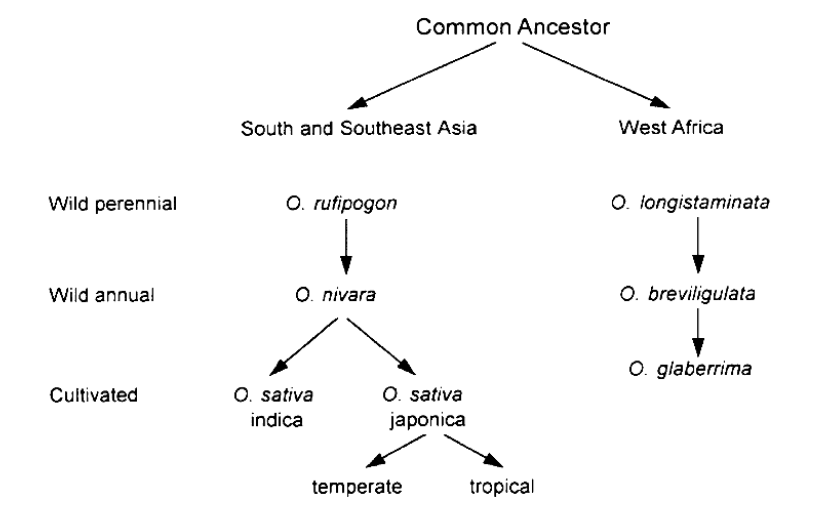
\includegraphics[width=0.9\linewidth]{./../images/cultivated-rice-type-evolution} \caption{Origins of cultivated \textit{Oryza} rice}\label{fig:cultivated-rice-evolution}
\end{figure}

\column{0.5\textwidth}

\begin{figure}
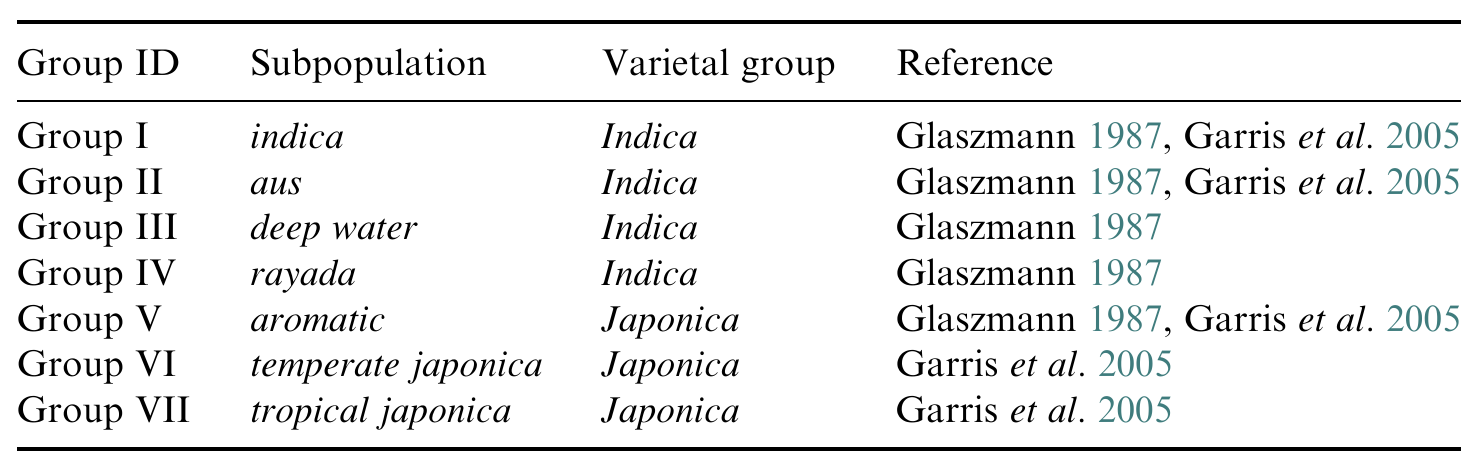
\includegraphics[width=0.99\linewidth]{./../images/rice_subpopulations} \caption{The recognized subpopulations of \textit{Oryza sativa}}\label{fig:subpopulations-rice}
\end{figure}

\end{columns}
\end{frame}

\begin{frame}{}
\protect\hypertarget{section-15}{}
\begin{itemize}
\tightlist
\item
  First archaeological evidence of rice cultivation leads to Yangtze
  valley of eastern China.
\item
  Domestication has resulted in alterations to a large array of
  morphological traits:

  \begin{itemize}
  \tightlist
  \item
    Seed shattering behavior
  \item
    Grain coloration
  \item
    Grain size enlargement
  \item
    Prostrate to erect growth habit
  \item
    Reduced seed dormancy
  \end{itemize}
\item
  Genetic factors contributing to domestication syndrome
  \emph{Shattering4 (Sha4)} on chromosome 4 and black hull by
  \emph{Black hull (Bh4)} on chromosome 4.
\end{itemize}
\end{frame}

\begin{frame}{Maize}
\protect\hypertarget{maize}{}
\begin{itemize}
\tightlist
\item
  Domestication history based on 7100 year old maize pollen from San
  Andres.
\item
  Initially cultivated in seasonal tropical forest of southwestern
  mexico.
\item
  Originated from annual teosinte (\emph{Zea mays} subspecies
  \emph{parviglumis}) around 9000 years ago in mid to lowland regions.
\item
  Later on admixture occured among \emph{parviglumis} and
  \emph{mexicana} (highland type) subspecies.
\end{itemize}
\end{frame}

\begin{frame}{Wheat}
\protect\hypertarget{wheat}{}
\begin{figure}
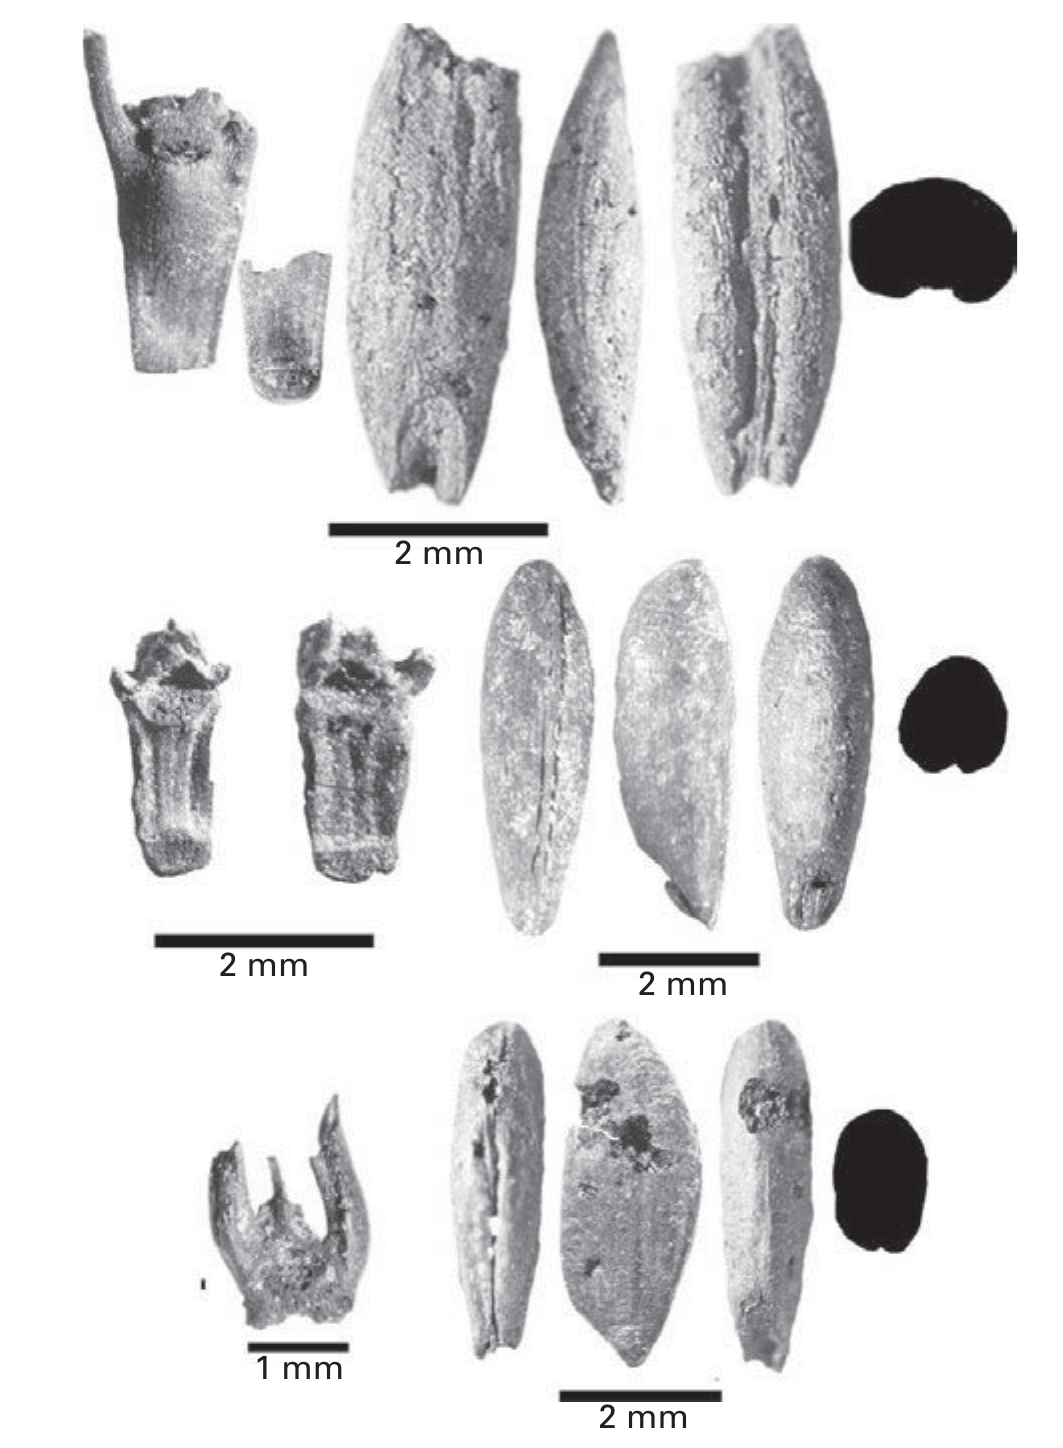
\includegraphics[width=0.32\linewidth]{./../images/charred_grass_grains} \caption{Charred wild cereal spikelet bases (left) and grains (right). Top, Hordeum spontaneum (wild barley) from Jerf el Ahmar. Middle, Secale sp. (rye) from Jerf el Ahmar. Bottom, Triticum boeoticum (single-grain einkorn) from Tell Qaramel. Note the basal abscission scar seen in the barley (top row, second from the left) and for rye the lower end of the rye spikelet bases (second row, first and second from left) is more reliable than the upper scar for distinguishing between wild and domestic.}\label{fig:wheat-barley-archaeology}
\end{figure}
\end{frame}

\hypertarget{megacentres-of-cutivated-plants}{%
\subsection{Megacentres of cutivated
plants}\label{megacentres-of-cutivated-plants}}

\begin{frame}{}
\protect\hypertarget{section-16}{}
\begin{figure}
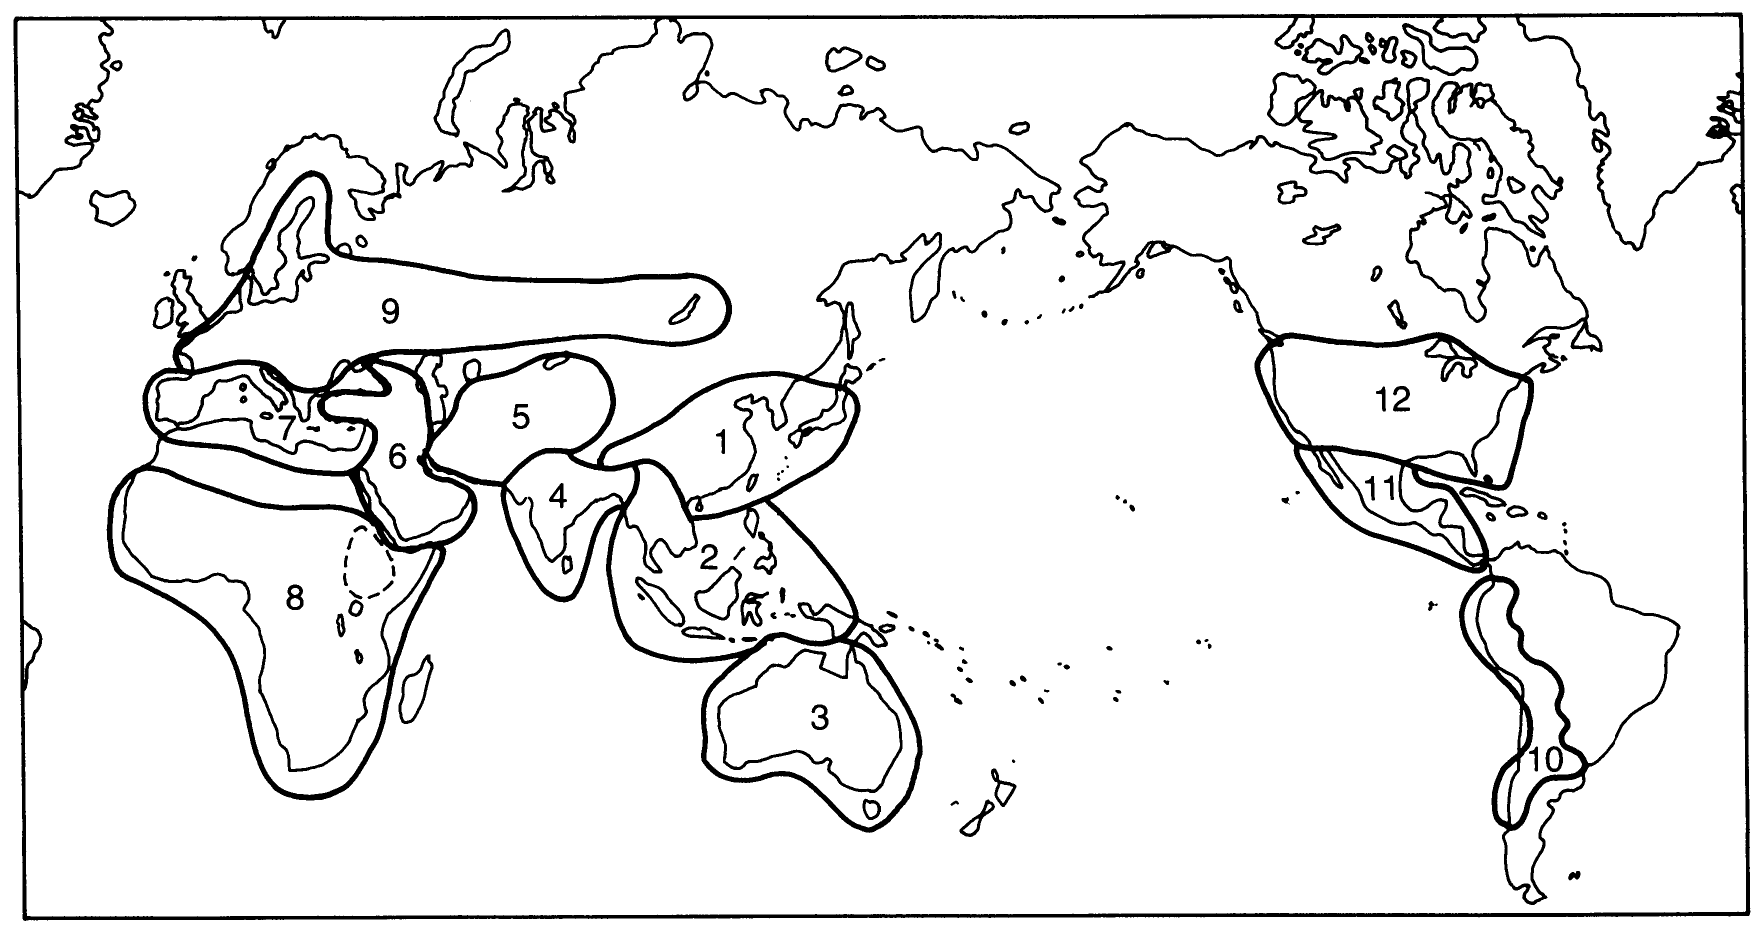
\includegraphics[width=0.6\linewidth]{./../images/megacentres_cultivated} \caption{Megacentres of cultivated plants (Zeven and Zhukovsky, 1975); @hayward2012plant, Page 37}\label{fig:cultivated-megacentres}
\end{figure}
\end{frame}

\begin{frame}{}
\protect\hypertarget{section-17}{}
\begin{table}

\caption{\label{tab:diversity-region1}Cultivated plants and their regions of diversity. Based on Zeven and Zhukovsky (1975) and Zeven and de Wet (1982); @hayward2012plant, Page 54, 55.}
\centering
\fontsize{6}{8}\selectfont
\begin{tabular}[t]{>{\raggedright\arraybackslash}p{3em}>{\raggedright\arraybackslash}p{14em}>{\raggedright\arraybackslash}p{32em}}
\toprule
SN & Region & Crops\\
\midrule
\textbf{\cellcolor{gray!6}{1}} & \cellcolor{gray!6}{Chinese-Japanese region} & \cellcolor{gray!6}{Prosomillet, Foxtail millet, Naked oat}\\
\textbf{} &  & Soybean, Adzuki bean\\
\textbf{\cellcolor{gray!6}{}} & \cellcolor{gray!6}{} & \cellcolor{gray!6}{Leafy mustard}\\
\textbf{} &  & Orange/Citrus, Peach, Apricot, Litchi\\
\textbf{\cellcolor{gray!6}{}} & \cellcolor{gray!6}{} & \cellcolor{gray!6}{Bamboo, Ramie, Tung oil tree, Tea}\\
\addlinespace
\textbf{2} & Indochinese-Indonesian region & Rice\\
\textbf{\cellcolor{gray!6}{}} & \cellcolor{gray!6}{} & \cellcolor{gray!6}{Rice bean, Winged bean}\\
\textbf{} &  & Cucurbits/Ash gourd\\
\textbf{\cellcolor{gray!6}{}} & \cellcolor{gray!6}{} & \cellcolor{gray!6}{Mango, Banana, Rambutan, Durian, Bread fruit, Citrus/Lime, Grapefruit}\\
\textbf{} &  & Bamboos, Nutmeg, Clove, Sago-palm, Ginger, Taros and Yams, Betel nut, Coconut\\
\addlinespace
\textbf{\cellcolor{gray!6}{3}} & \cellcolor{gray!6}{Australian region} & \cellcolor{gray!6}{Eucalyptus, Acacia, Macadamia nut}\\
\textbf{4} & Hindustani region & Rice, Little millet\\
\textbf{\cellcolor{gray!6}{}} & \cellcolor{gray!6}{} & \cellcolor{gray!6}{Black gram, Green gram, Moth bean, Rice bean, Dolichos bean, Pigeonpea, Cowpea, Chickpea, Horsegram, Jute}\\
\textbf{} &  & Eggplant, Okra, Cucumber, Leafy mustard, Rat's tail radish, Taros and Yams\\
\textbf{\cellcolor{gray!6}{}} & \cellcolor{gray!6}{} & \cellcolor{gray!6}{Citrus, Banana, Mango, Sunhemp, Tree cotton}\\
\bottomrule
\end{tabular}
\end{table}
\end{frame}

\begin{frame}{}
\protect\hypertarget{section-18}{}
\begin{table}

\caption{\label{tab:diversity-region2}Cultivated plants and their regions of diversity. Based on Zeven and Zhukovsky (1975) and Zeven and de Wet (1982); @hayward2012plant, Page 54, 55.}
\centering
\fontsize{6}{8}\selectfont
\begin{tabular}[t]{>{\raggedright\arraybackslash}p{3em}>{\raggedright\arraybackslash}p{14em}>{\raggedright\arraybackslash}p{32em}}
\toprule
SN & Region & Crops\\
\midrule
\textbf{\cellcolor{gray!6}{}} & \cellcolor{gray!6}{} & \cellcolor{gray!6}{Sesame, Ginger, Turmeric, Cardamom, Arecanut, Sugarcane, Black pepper, Indigo}\\
\textbf{5} & Central Asian region & Wheat (Bread/Club/Shot), Rye\\
\textbf{\cellcolor{gray!6}{}} & \cellcolor{gray!6}{} & \cellcolor{gray!6}{Allium/Onion, Garlic, Spinach, Peas, Beetroot, Faba bean}\\
\textbf{} &  & Lentil, Chickpea\\
\textbf{\cellcolor{gray!6}{}} & \cellcolor{gray!6}{} & \cellcolor{gray!6}{Apricot, Plum, Pear, Apple, Walnut, Almond, Pistachio, Melon, Grape, Carrot, Radish}\\
\addlinespace
\textbf{} &  & Hemp/Cannabis, Sesame, Flax, Safflower\\
\textbf{\cellcolor{gray!6}{6}} & \cellcolor{gray!6}{Near Eastern region} & \cellcolor{gray!6}{Wheat (Einkorn, Durum, Poulard, Bread), Barley, Rye/Secale}\\
\textbf{} &  & Faba bean, Chickpea, French bean, Lentil, Pea\\
\textbf{\cellcolor{gray!6}{}} & \cellcolor{gray!6}{} & \cellcolor{gray!6}{Brassica oleracea, Allium, Melon, Grape, Plum, Pear, Apple, Apricot, Pistachio, Fig, Pomegranate, Almond}\\
\textbf{} &  & Safflower, Sesame, Flax\\
\addlinespace
\textbf{\cellcolor{gray!6}{}} & \cellcolor{gray!6}{} & \cellcolor{gray!6}{Lupins, Medics}\\
\textbf{7} & Mediterranean region & Wheat (Durum, Turgidum), Oats\\
\textbf{\cellcolor{gray!6}{}} & \cellcolor{gray!6}{} & \cellcolor{gray!6}{Brassica oleracea, Lettuce, Beetroot, Colza}\\
\textbf{} &  & Faba bean, Radish\\
\textbf{\cellcolor{gray!6}{}} & \cellcolor{gray!6}{} & \cellcolor{gray!6}{Olive, Trifolium/Berseem, Lupins, Crocus, Grape, Fennel, Cumin, Celery, Linseed}\\
\bottomrule
\end{tabular}
\end{table}
\end{frame}

\begin{frame}{}
\protect\hypertarget{section-19}{}
\begin{table}

\caption{\label{tab:diversity-region3}Cultivated plants and their regions of diversity. Based on Zeven and Zhukovsky (1975) and Zeven and de Wet (1982); @hayward2012plant, Page 54, 55.}
\centering
\fontsize{6}{8}\selectfont
\begin{tabular}[t]{>{\raggedright\arraybackslash}p{3em}>{\raggedright\arraybackslash}p{14em}>{\raggedright\arraybackslash}p{32em}}
\toprule
SN & Region & Crops\\
\midrule
\textbf{\cellcolor{gray!6}{8}} & \cellcolor{gray!6}{African region} & \cellcolor{gray!6}{Wheat (Durum, Emmer, Poulard, Bread)}\\
\textbf{} &  & African rice, Sorghum, Pearl millet, Finger millet, Teff\\
\textbf{\cellcolor{gray!6}{}} & \cellcolor{gray!6}{} & \cellcolor{gray!6}{Cowpea, Bottle gourd, Okra, Yams, Cucumber}\\
\textbf{} &  & Castor bean, Sesame, Niger, Oil palm, Safflower, Flax\\
\textbf{\cellcolor{gray!6}{}} & \cellcolor{gray!6}{} & \cellcolor{gray!6}{Cotton, Kenaf, Coffee}\\
\addlinespace
\textbf{} &  & Kola, Bambara, Groundnut, Date palm, Ensete, Melons\\
\textbf{\cellcolor{gray!6}{9}} & \cellcolor{gray!6}{European-siberian region} & \cellcolor{gray!6}{Peach, Pear, Plum, Apricot, Apple, Almond, Walnut, Pistachio, Cherry}\\
\textbf{} &  & Cannabis, Mustard (black), Chicory, Hops, Lettuce\\
\textbf{\cellcolor{gray!6}{10}} & \cellcolor{gray!6}{South American region} & \cellcolor{gray!6}{Potato, Sweet potato, Xanthosoma}\\
\textbf{} &  & Lima bean, Amaranth, Chenopodium, Cucurbita, Tomato, Tobacco, Lupin\\
\addlinespace
\textbf{\cellcolor{gray!6}{}} & \cellcolor{gray!6}{} & \cellcolor{gray!6}{Papaya, Pineapple}\\
\textbf{} &  & Groundnut, Sea island cotton\\
\textbf{\cellcolor{gray!6}{}} & \cellcolor{gray!6}{} & \cellcolor{gray!6}{Cassava, Cacao, Rubber tree, Passion fruit}\\
\textbf{11} & Central American and Mexican region & Maize, French bean, Potato, Cucurbita, Pepper/Chilli, Amaranth, Chenopodium, Tobacco, Sisal hemp, Upland cotton\\
\textbf{\cellcolor{gray!6}{12}} & \cellcolor{gray!6}{North American region} & \cellcolor{gray!6}{Jeruselum artichoke, Sunflower, Plum, Raspberry, Strawberry}\\
\bottomrule
\end{tabular}
\end{table}
\end{frame}

\hypertarget{plant-introduction}{%
\subsection{Plant introduction}\label{plant-introduction}}

\begin{frame}{Background}
\protect\hypertarget{background}{}
\begin{itemize}
\item
  The plant breeder may import new, unadapted genotypes from outside the
  production region, usually from another country (called plant
  introductions). These new materials may be evaluated and adapted to
  new production regions as new cultivars, or used as parents for
  crossing in breeding projects.
\item
  Primary Introduction

  \begin{itemize}
  \tightlist
  \item
    When the introduced variety is well adapted to the new environment,
    it is released for commercial cultivating without any alteration in
    the original genotype; this constitutes primary introduction. It is
    less common, particularly in countries having well organized crop
    improvement programmes.
  \end{itemize}
\item
  Secondary introduction

  \begin{itemize}
  \tightlist
  \item
    The introduced variety may be subject to selection in order to
    isolate a superior variety. Alternatively, it may be hybridized with
    local varieties to transfer one or few characters from these
    varieties to the local ones. Such introduction constitutes secondary
    introduction. It is much common than primary introduction.
  \end{itemize}
\end{itemize}
\end{frame}

\begin{frame}{Purpose}
\protect\hypertarget{purpose}{}
\begin{enumerate}
\tightlist
\item
  To obtain entirely new crop species
\item
  To serve as new varieties
\item
  For use in crop improvement programmes
\item
  To introgress variability to existing genetic materials
\item
  For scientific studies
\item
  To augment aesthetics
\item
  For germplasm collection and comparison
\end{enumerate}
\end{frame}

\hypertarget{bibliography}{%
\section*{Bibliography}\label{bibliography}}
\addcontentsline{toc}{section}{Bibliography}

\begin{frame}{Bibliography}
\hypertarget{refs}{}
\begin{cslreferences}
\leavevmode\hypertarget{ref-barron2020snapshots}{}%
Barron, Aleese, Dorian Q Fuller, Chris Stevens, Louis Champion, Frank
Winchell, and Tim Denham. 2020. ``Snapshots in Time: MicroCT Scanning of
Pottery Sherds Determines Early Domestication of Sorghum (Sorghum
Bicolor) in East Africa.'' \emph{Journal of Archaeological Science} 123:
105259.

\leavevmode\hypertarget{ref-fuller2009domestication}{}%
Fuller, Dorian Q, Ling Qin, Yunfei Zheng, Zhijun Zhao, Xugao Chen, Leo
Aoi Hosoya, and Guo-Ping Sun. 2009. ``The Domestication Process and
Domestication Rate in Rice: Spikelet Bases from the Lower Yangtze.''
\emph{Science} 323 (5921): 1607--10.

\leavevmode\hypertarget{ref-wu2017single}{}%
Wu, Wenguang, Xiaoyun Liu, Muhua Wang, Rachel S Meyer, Xiaojin Luo,
Marie-Noelle Ndjiondjop, Lubin Tan, et al. 2017. ``A Single-Nucleotide
Polymorphism Causes Smaller Grain Size and Loss of Seed Shattering
During African Rice Domestication.'' \emph{Nature Plants} 3 (6): 1--7.
\end{cslreferences}
\end{frame}

\end{document}
